
% --------------------------------------------------------------------------------------------------
% Kommando Beispiele
% --------------------------------------------------------------------------------------------------

% Referenz auf z.B. Kapitel
\chapter{Template}
\label{c:template}

Start writing here \ref{c:template}...

% Einfaches Bild
% 
% [scale=0.5]
% [width=1.0\textwidth]
\begin{figure}[htbp]
  \centering
  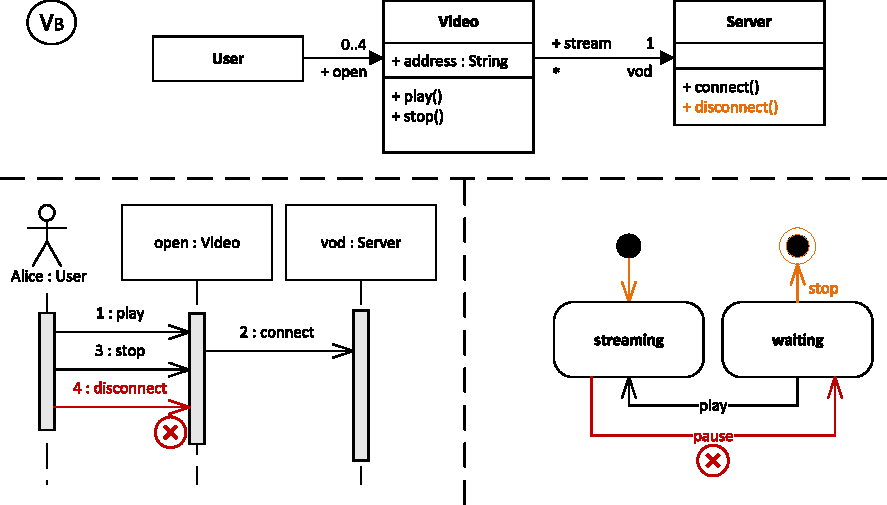
\includegraphics[width=1.0\textwidth]{figures/example_model01.pdf}
  \caption{Figure description here}
  \label{fig:model}
\end{figure}

% Referenz auf Bild
Figure \ref{fig:model}

% List
\begin{itemize}
  \item one
  \item two
\end{itemize}

% Aufzählung
\begin{enumerate}
  \item one
  \item two
\end{enumerate}

In Definition \ref{def:emc}...

% Theorem Style
\begin{definition}\label{def:emc} $e=mc^2$ \end{definition}
\begin{lemma} $e=mc^2$ \end{lemma}
\begin{proof} $e=mc^2$ \end{proof}
\begin{requirement} $e=mc^2$ \end{requirement}
\begin{example} $e=mc^2$ \end{example}

% Java Code
\begin{lstlisting}[float=tbh, mathescape=true, captionpos=b, caption=foo, label=bar]
  // Hello.java
  import java.awt.Graphics;
  public class Hello extends JApplet {}
\end{lstlisting}

% Pseudo Code
\begin{lstlisting}[float=tbh, mathescape=true, captionpos=b, caption=foo, label=pseudo_code, language=pseudo]
  function helloWorld(in name) {}
\end{lstlisting}

% Noch zu Erledigen Hinweis
\todo{HERE A TODO!}

% Randnotiz
\notiz{SOME NOTE}

% Struktur
\section{Section}
\subsection{SubSection}
\subsubsection{SubSubSection}
\paragraph{Pragraph}
\subparagraph{SubPragraph}
